\documentclass[a4paper,12pt]{article}
\usepackage[
top=2.5cm,
bottom=2.5cm,
left=2cm,
right=2cm,
]{geometry}

\usepackage{enumitem}
\usepackage{amsmath,amssymb,latexsym}
\usepackage{pifont}

% Automata
\usepackage{tikz}
\usetikzlibrary{ arrows, automata, bbox, positioning}
\tikzset{
->, % makes the edges directed
>=stealth', % makes the arrow heads bold
node distance=3cm, % specifies the minimum distance between two nodes. Change if necessary.
every state/.style={thick}, % sets the properties for each ’state’ node
initial text=Start, % sets the text that appears on the start arrow
}

% Tree
\usepackage{forest}

% Side by side figure
\usepackage{subcaption}

% No indentation
\setlength\parindent{0pt}

% Put figure at the top of a page when its on a new page
\makeatletter
\setlength{\@fptop}{0pt}
\makeatother
%

% Shorthand
\newcommand{\s}[1]{s_{#1}}
\newcommand{\caps}[1]{S_{#1}}
\newcommand{\ntxt}[1]{\footnotesize{#1}}
\newcommand{\cpp}{\small{\texttt{<<}}}


\begin{document}
\section{NFA to DFA}
In the following table, initial state is labeled with \(\rightarrow\) and final states are labeled with \(*\).
% The height of each row is set to 1.2 relative to its default height.
\renewcommand{\arraystretch}{1.2}
\begin{table}[h]
\centering
\begin{tabular}[tb]{r||l|l}
   state & 0 & 1 \\
  \hline
  \(\varnothing\) & \(\varnothing\) & \(\varnothing\) \\

  \(\rightarrow \{\s{0}\}\) & \(\varnothing\) & \(\{\s{1}\}\)\\

  \(\{\s{1}\}\) & \(\{\s{1}, \s{3}\}\) & \(\{\s{2}, \s{4}\}\) \\

  \(*\{\s{2}\}\) & \(\{\s{2}, \s{4}\}\) & \(\{\s{2}\}\) \\

  \(\{\s{3}\}\) & \(\{\s{4}\}\) & \(\{\s{0}, \s{3}\}\) \\

  \(\{\s{4}\}\) & \(\varnothing\) & \(\varnothing\) \\

  \(\{\s{1}, \s{3}\}\) & \(\{\s{1}, \s{3}, \s{4}\}\) & \(\{\s{0}, \s{2}, \s{3}, \s{4}\}\) \\

  \(*\{\s{2}, \s{4}\}\) & \(\{\s{2}, \s{4}\}\) & \(\{\s{2}\}\) \\

  \(\{\s{0}, \s{3}\}\) & \(\{\s{4}\}\) & \(\{\s{0}, \s{1}, \s{3}\}\) \\

  \(\{\s{1}, \s{3}, \s{4}\}\) & \(\{\s{1}, \s{3}, \s{4}\}\) & \(\{\s{0}, \s{2}, \s{3}, \s{4}\}\) \\

  \(*\{\s{0}, \s{2}, \s{3}, \s{4}\}\) & \(\{\s{2}, \s{4}\}\) & \(\{\s{0}, \s{1}, \s{2}, \s{3}\}\) \\

  \(\{\s{0}, \s{1}, \s{3}\}\) & \(\{\s{1}, \s{3}, \s{4}\}\) & \(\{\s{0}, \s{1}, \s{2}, \s{3}, \s{4}\}\) \\

  \(*\{\s{0}, \s{1}, \s{2}, \s{3}\}\) & \(\{\s{1}, \s{2}, \s{3}, \s{4}\}\) & \(\{\s{0}, \s{1}, \s{2}, \s{3}, \s{4}\}\) \\

  \(*\{\s{0}, \s{1}, \s{2}, \s{3}, \s{4}\}\) & \(\{\s{1}, \s{2}, \s{3}, \s{4}\}\) & \(\{\s{0}, \s{1}, \s{2}, \s{3}, \s{4}\}\) \\

  \(*\{\s{1}, \s{2}, \s{3}, \s{4}\}\) & \(\{\s{1}, \s{2}, \s{3}, \s{4}\}\) & \(\{\s{0}, \s{2}, \s{3}, \s{4}\}\) \\
\end{tabular}
\caption{The subset construction}
\end{table}

\section{DFA minimisation}
\renewcommand{\labelitemii}{\ding{226}}
\begin{enumerate}
% initial split
\item initial split: \(\{\s{1},\s{5}\}\), \(\{\s{0}, \s{2}, \s{3}, \s{4}\}\)
  \begin{itemize}
    \item check \(\{\s{1},\s{5}\}\)
      \begin{itemize}
      \item \(\s{1} \overset{0}{\rightarrow} \s{2}\), second group
      \item \(\s{5} \overset{0}{\rightarrow} \s{0}\), second group
      \item \(\s{1} \overset{1}{\rightarrow} \s{1}\), first group
      \item \(\s{5} \overset{1}{\rightarrow} \s{1}\), first group
      \item[] no split
    \end{itemize}

    \item check \(\{\s{0}, \s{2}, \s{3}, \s{4}\}\)
      \begin{itemize}
      \item \(\s{0} \overset{0}{\rightarrow} \s{1}\), first group
      \item \(\s{2} \overset{0}{\rightarrow} \s{5}\), first group
      \item \(\s{3}/\s{4} \overset{0}{\rightarrow} \s{4}\), second group
      \item \(\s{3} \overset{1}{\rightarrow} \s{3}\), second group
      \item \(\s{4} \overset{1}{\rightarrow} \s{0}\), first group
      \item[] split out \(\s{3}\) and \(\s{4}\)
    \end{itemize}
\end{itemize}

% 2nd split
\item next split: \(\{\s{1},\s{5}\}\), \(\{\s{0}, \s{2}\}\), \(\{\s{3}\}\), \(\{\s{4}\}\)
  \begin{itemize}
  \item check \(\{\s{1},\s{5}\}\)
    \begin{itemize}
      \item \(\s{1} \overset{0}{\rightarrow} \s{2}\), second group
      \item \(\s{5} \overset{0}{\rightarrow} \s{0}\), second group
      \item \(\s{1}/\s{5} \overset{1}{\rightarrow} \s{1}\), first group
      \item [] no split
    \end{itemize}
  \item check \(\{\s{0}, \s{2}\}\)
    \begin{itemize}
      \item \(\s{0} \overset{0}{\rightarrow} \s{1}\), first group
      \item \(\s{2} \overset{0}{\rightarrow} \s{5}\), first group
      \item \(\s{0}/\s{2} \overset{1}{\rightarrow} \s{3}\), third group
      \item[] no split
    \end{itemize}
  \item no need to check \(\{\s{3}\}\) or \(\{\s{4}\}\) alone
  \end{itemize}
\item Merge \(\s{1}\) and \(\s{5}\)
\item Merge \(\s{0}\) and \(\s{2}\)
\item Finally got \(\s{0}, \s{1}, \s{3}, \s{4}\)
\end{enumerate}

\section{\(\epsilon\)-NFA to NFA}
\subsection{\(\epsilon\)-closure}
\textbf{Solution.}
% step 1 find eclose of all states
\begin{itemize}
\item ECLOSE\((\s{0})\) = \(\{\s{0}, \s{1}, \s{4}, \s{2}\}\)
\item ECLOSE\((\s{1})\) = \(\{\s{1}, \s{4}, \s{2}, \s{0}\}\)
\item ECLOSE\((\s{2})\) = \(\{\s{2}\}\)
\item ECLOSE\((\s{3})\) = \(\{\s{3}\}\)
\item ECLOSE\((\s{4})\) = \(\{\s{4}, \s{2}, \s{0}, \s{1}\}\)
\end{itemize}
\subsection{Final NFA diagram}
\textbf{Solution.}\\
See diagram \ref{fig:nfa} on the next page.
% step 3 NFA
\clearpage
\begin{figure}[t]
  \centering
  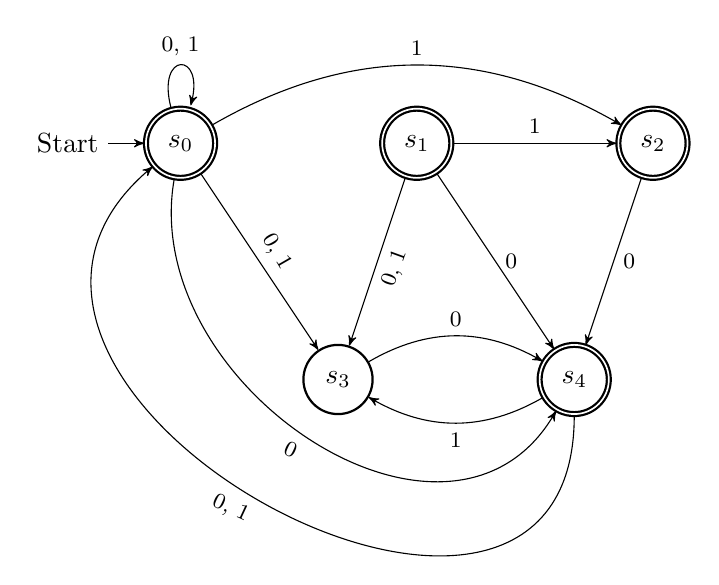
\begin{tikzpicture}[bezier bounding box]% reduce vertical spacing after tikzpicture
  \node[state, initial, accepting] (s0) {\(\s{0}\)};
  \node[state, accepting, right of=s0] (s1) {\(\s{1}\)};
  \node[state, accepting, right of=s1] (s2) {\(\s{2}\)};
  \node[state, right of=s0, xshift=-1cm, yshift=-3cm] (s3) {\(\s{3}\)};
  \node[state, accepting, right of=s3] (s4) {\(\s{4}\)};

  \draw (s0) edge[loop above] node{\ntxt{0, 1}} (s0)
             edge[bend left, above] node{\ntxt{1}} (s2)
             edge[above] node[rotate=-60]{\ntxt{0, 1}} (s3)
             edge[out=-100, in=-120, looseness=1.2] node[below left, rotate=-25]{\ntxt{0}} (s4)
        (s1) edge[above] node{\ntxt{1}} (s2)
             edge[below, right=0.3] node{\ntxt{0}} (s4)
             edge[below, right=0.3] node[below, rotate=70]{\ntxt{0, 1}} (s3)
        (s2) edge[below, right=0.3] node{\ntxt{0}} (s4)
        (s3) edge[bend left, above] node{\ntxt{0}} (s4)
        (s4) edge[bend left] node[below]{\ntxt{1}} (s3)
             edge[out=-90, in=-140, looseness=1.8] node[below left, rotate=-25]{\ntxt{0, 1}} (s0);
  \end{tikzpicture}
  \caption{NFA without \(\epsilon\)}
  \label{fig:nfa}
\end{figure}

\section{C++ streams}
\textbf{Solution}.
The grammar can be expressed using the following productions:
\begin{enumerate}[noitemsep]
\item \(S \rightarrow S\; \cpp\; S\)
\item \(S \rightarrow O\)
\item \(O \rightarrow \texttt{ostream}\)
\item \(O \rightarrow \texttt{string}\)
\item \(O \rightarrow \texttt{int}\)
\end{enumerate}
\subsection{Leftmost derivation One}
% TODO: figure out how to use the format in automata theory 3rd, pp178
\begin{align*}
S & \Rightarrow S\; \cpp\; S && \text{Production 1}  \\
  & \Rightarrow O\; \cpp\; S && \text{Production 2} \\
  & \Rightarrow \texttt{ostream}\; \cpp\; S\; && \text{Production 3} \\
  & \Rightarrow \texttt{ostream}\; \cpp\; S\; \cpp\; S  && \text{Production 1} \\
  & \Rightarrow \texttt{ostream}\; \cpp\; O\; \cpp\; S  && \text{Production 2} \\
  & \Rightarrow \texttt{ostream}\; \cpp\; \texttt{string}\; \cpp\; S  && \text{Production 4} \\
  & \Rightarrow \texttt{ostream}\; \cpp\; \texttt{string}\; \cpp\; O && \text{Production 2} \\
  & \Rightarrow \texttt{ostream}\; \cpp\; \texttt{string}\; \cpp\; \texttt{int} && \text{Production 5}
\end{align*}
\subsection{Leftmost derivation Two}
\begin{align*}
S & \Rightarrow S\; \cpp\; S && \text{Production 1}  \\
  & \Rightarrow S\; \cpp\; S\; \cpp\; S && \text{Production 1} \\
  & \Rightarrow O\; \cpp\; S\; \cpp\; S && \text{Production 2} \\
  & \Rightarrow O\; \cpp\; O\; \cpp\; S && \text{Production 2} \\
  & \Rightarrow O\; \cpp\; O\; \cpp\; O && \text{Production 2} \\
  & \Rightarrow \texttt{ostream}\; \cpp\; O\; \cpp\; O  && \text{Production 3} \\
  & \Rightarrow \texttt{ostream}\; \cpp\; \texttt{string}\; \cpp\; O  && \text{Production 4} \\
  & \Rightarrow \texttt{ostream}\; \cpp\; \texttt{string}\; \cpp\; \texttt{int}  && \text{Production 5}
\end{align*}
\subsection{Associative}
\textbf{Solution}.
The binary operator \cpp should be left associative, i.e
\[
\texttt{ostream << string << int} = \texttt{(ostream << string) << int}
\]
The reasons I can think of are:
\begin{enumerate}
\item It is \emph{intuitive}, the execution order is the same as that of writing, from left to right
\item \cpp outputs its right argument as a side effect, hence right-associativity will cause its right argument to be output first, which is \emph{not} the desired result.  For example:
  \begin{enumerate}
  \item ``\texttt{This is a short line} \verb|\n|'' will output each word in a reverse order; The linebreak character ``\verb|\n|'' will be output first
  \item ``\texttt{3}'' \cpp ``\texttt{3}'' \cpp ``\texttt{1}'' \cpp ``\texttt{=}'' \cpp ``\texttt{4}'' may first output \texttt{ 1 = 4} (very confusing) if the outputing is done on a quite slow machine
  \end{enumerate}
\end{enumerate}
\subsection{Unambiguous}
\textbf{Solution}.\\
Add a new variable \emph{term} (denoted as \(T\)) to the original grammar.  \(T\) is an expression that cannot be broken apart by any \cpp on its right side.

With \(T\), the grammar now becomes:
\begin{itemize}[itemsep=0pt]
\item[] \(O\; \rightarrow\; \texttt{ostream}\; |\; \texttt{string}\; |\; \texttt{int} \)
\item[] \(T\; \rightarrow\; O \;|\; T\; \cpp\; O\)
\item[] \(S\; \rightarrow\; T \;|\; T\; \cpp\; S\)
\end{itemize}
\begin{align*}
\end{align*}
The fact that grammar is unambiguous can be observed from the parse trees of \(T\) and \(S\) respectively:
\begin{figure}[t!]
  \centering
  % Parse tree of T
  \subcaptionbox{Parse tree of \(T\)}
  [0.4\linewidth]{
  \begin{forest}
      [T
        [T
        [T
        [T
        [\dots
        [,phantom]
        [T
        [T [O]]
        [\cpp]
        [O]]
        ]]
        [\cpp]
        [O]]
        [\cpp]
        [O]]
        [O]
      ]
    \end{forest}
  }
  % Parse tree of S
  \subcaptionbox{Parse tree of \(S\)}
  [0.4\linewidth]{
    \begin{forest}
      [S
        [T [O]]
        [S
        [T [O]]
        [\cpp]
        [S
        [T [O]]
        [\cpp]
        [S
        [\dots
        [,phantom]
        [S
        [T [O]]
        [\cpp]
        [T [O]]]
        ]]]]
      ]
      \end{forest}
  }
  \caption{Parse trees}
\end{figure}

\section{Deterministic Context Free Languages}
\subsection{Associative}
\subsection{Unambiguous}
\end{document}
